\clearpage

\section{sgnToWfm}


\subsection*{Functional Description}

This Matlab function converts signals produced by the simulator (files with the extension .sgn) to waveforms  (files with the extension .wfm). This waveform files can be read, and later on, outputted by the Arbitrary Waveform Generator (AWG).
The AWG we will be using is the Tekatronix AWG70002A witch has the following key specifications:
\begin{figure}[h]
	\centering
	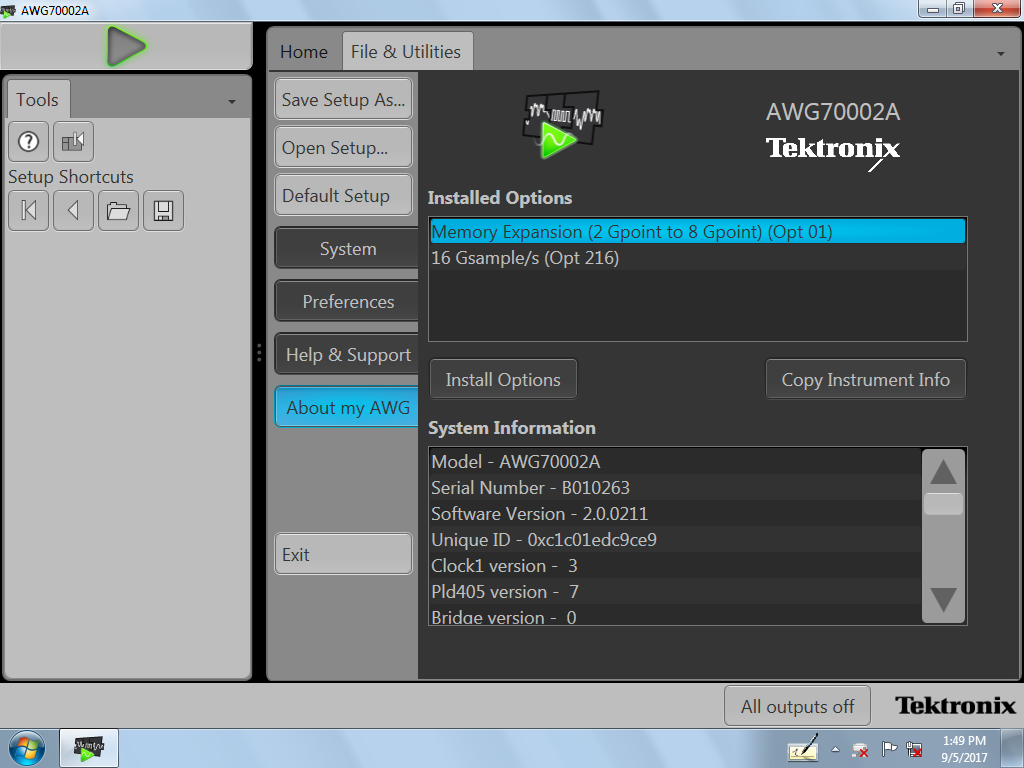
\includegraphics[width=\textwidth]{../mtools/sgnToWfm/figures/specs}
	\label{TUT_CompBad}\caption{AWG70002A key performance specifications}
\end{figure}
\bigskip

\textbf{Sampling rate up to 16 GS/s}: This is the most important spec because it determines the maximum sampling rate that your signal can have. It must not , in this case be over 16 GS/s or else the AWG will not be able to recreate it appropriately.

\textbf{8 GSample waveform memory}: This determines how many data points you can have in your signal. So your signal must not have more than 8G points.
\bigskip

\textbf{10 bit vertical resolution}: This determines how accurate the Digital to Analog converter is. The 10 bits corresponds to 1024 levels, considering that the max range of the signal peek to peek is 500 mV, then each level is separated by approximately 0.5 mV. You may also use 9 bits with 1 marker and 8 bits with 2 markers.
\bigskip



After making sure this specifications are respected you can create your waveform using this function. When you load your waveform, the AWG will output the waveform created and will repeat it constantly until you stop playing it.


\subsection*{Inputs}

The function requires only one input, a string with the name of the signal file that will be converted. 


\textbf{Type}: Real signal (ContinuousTimeContinuousAmplitudeReal)

\subsection*{Output}

If specified correctly the function will return six variables in the Matlab workspace, as well as creating a waveform file in the current folder.
Those variables are:

\bigskip

\textbf{data}: A vector with the waveform data.
\bigskip

\textbf{symbolPeriod}: Equal to the symbol period of the corresponding signal 
\bigskip

\textbf{samplingPeriod}: Sampling period of the signal.
\bigskip

\textbf{type}: A string with the name of the signal type. 
\bigskip

\textbf{numberOfSymbols}: Number of symbols retrieved from the signal.
\bigskip

\textbf{samplingRate}: This is equal to the sampling rate of the signal.
\bigskip

The samplingRate variable  should be noted as it will be important later on.

\subsection*{Tutorial - Loading a signal to the AWG}

\textbf{1. Using the function sgnToWfm}: 
Start up Matlab and change your current folder to mtools and add the signals folder that you want to convert to the Matlab search path. Use the function accordingly, putting as the input parameter the signal file you want to convert.


\noindent
\bigskip
\textbf{2. AWG sampling rate}: 
After calling the function there should be waveform file in the mtools folder, as well as a variable called samplingRate in the Matlab workspace. Make sure this is equal or bellow the maximum sampling frequency of the AWG (16 GS/s), or else the waveform can not be equal to the original signal. If it is higher you  have to adjust the parameters in the simulation in order to decrease the sampling frequency of the signal(i.e. decreasing the bit period or reducing the samples per symbol).
\bigskip

\noindent
\textbf{3. Loading the waveform file to the AWG}:
Copy the waveform file to your pen drive and connect it to the AWG. With the software of the awg open, go to browse waveforms, and select the waveform file you created (Figure 7.2).

\begin{figure}[h]
	\centering
	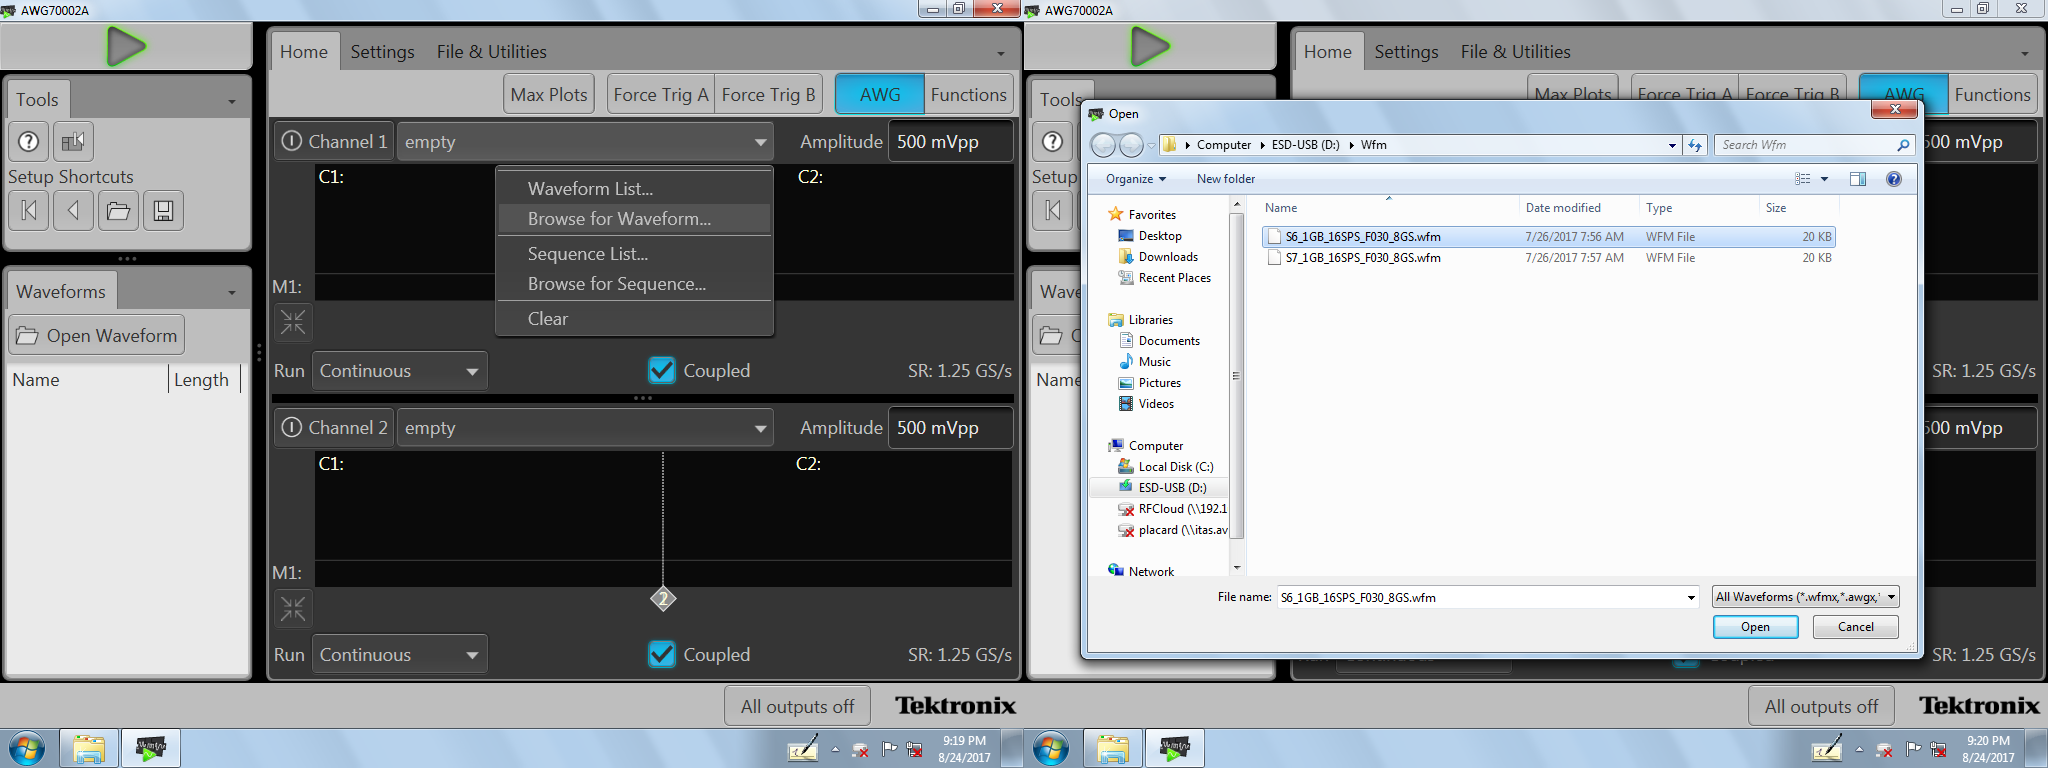
\includegraphics[width=\textwidth]{../mtools/sgnToWfm/figures/tutorial1}
	\label{TUT_SelectingWFM}\caption{Selecting your waveform in the AWG}
\end{figure}

Now you should have the waveform displayed on the screen. Although it has the same shape,  the waveform might not match the signal timing wise due to an incorrect sampling rate  configured in the AWG. 
In this example (Figure 7.3), the original signal has a sample rate of 8 GS/s and the AWG is configured to 1.25 GS/s. Therefore it must be changed to the correct value.

\begin{figure}[h]
	\centering
	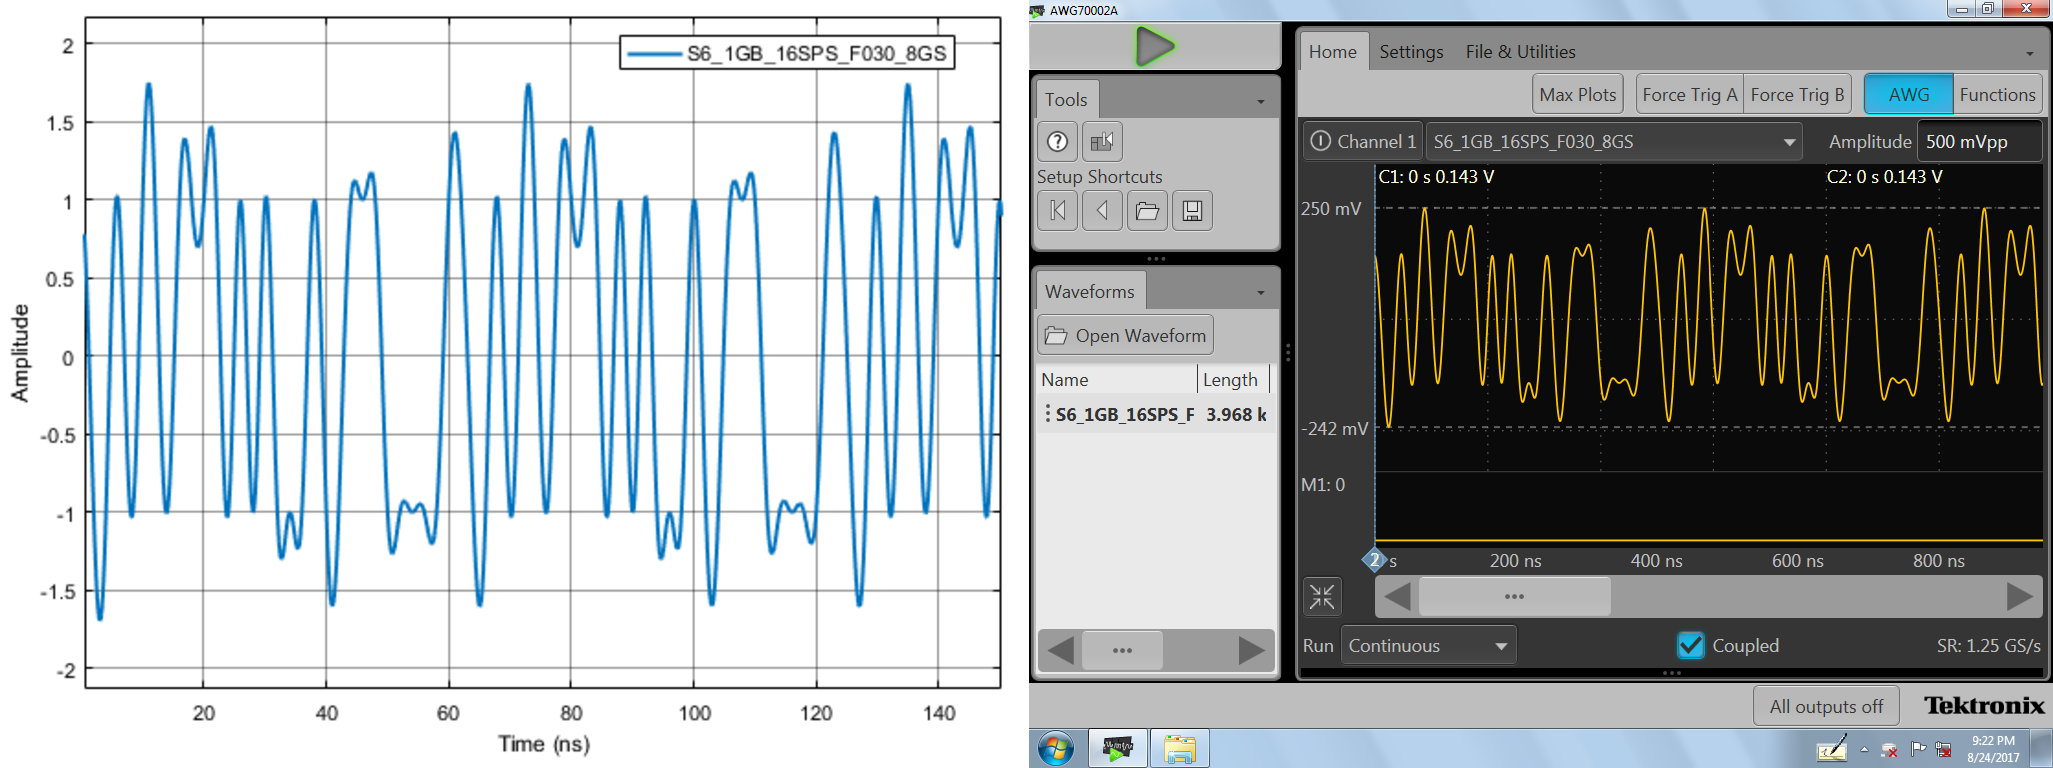
\includegraphics[width=\textwidth]{../mtools/sgnToWfm/figures/tutorial2}
	\label{TUT_CompBad}\caption{Comparison between the waveform in the AWG and the original signal before configuring the sampling rate}
\end{figure}
\bigskip
To do this go to the settings tab, clock settings, and change the sampling rate to be equal to the one of the original signal, 8 GS/s (Figure 7.4).

\begin{figure}[h]
	\centering
	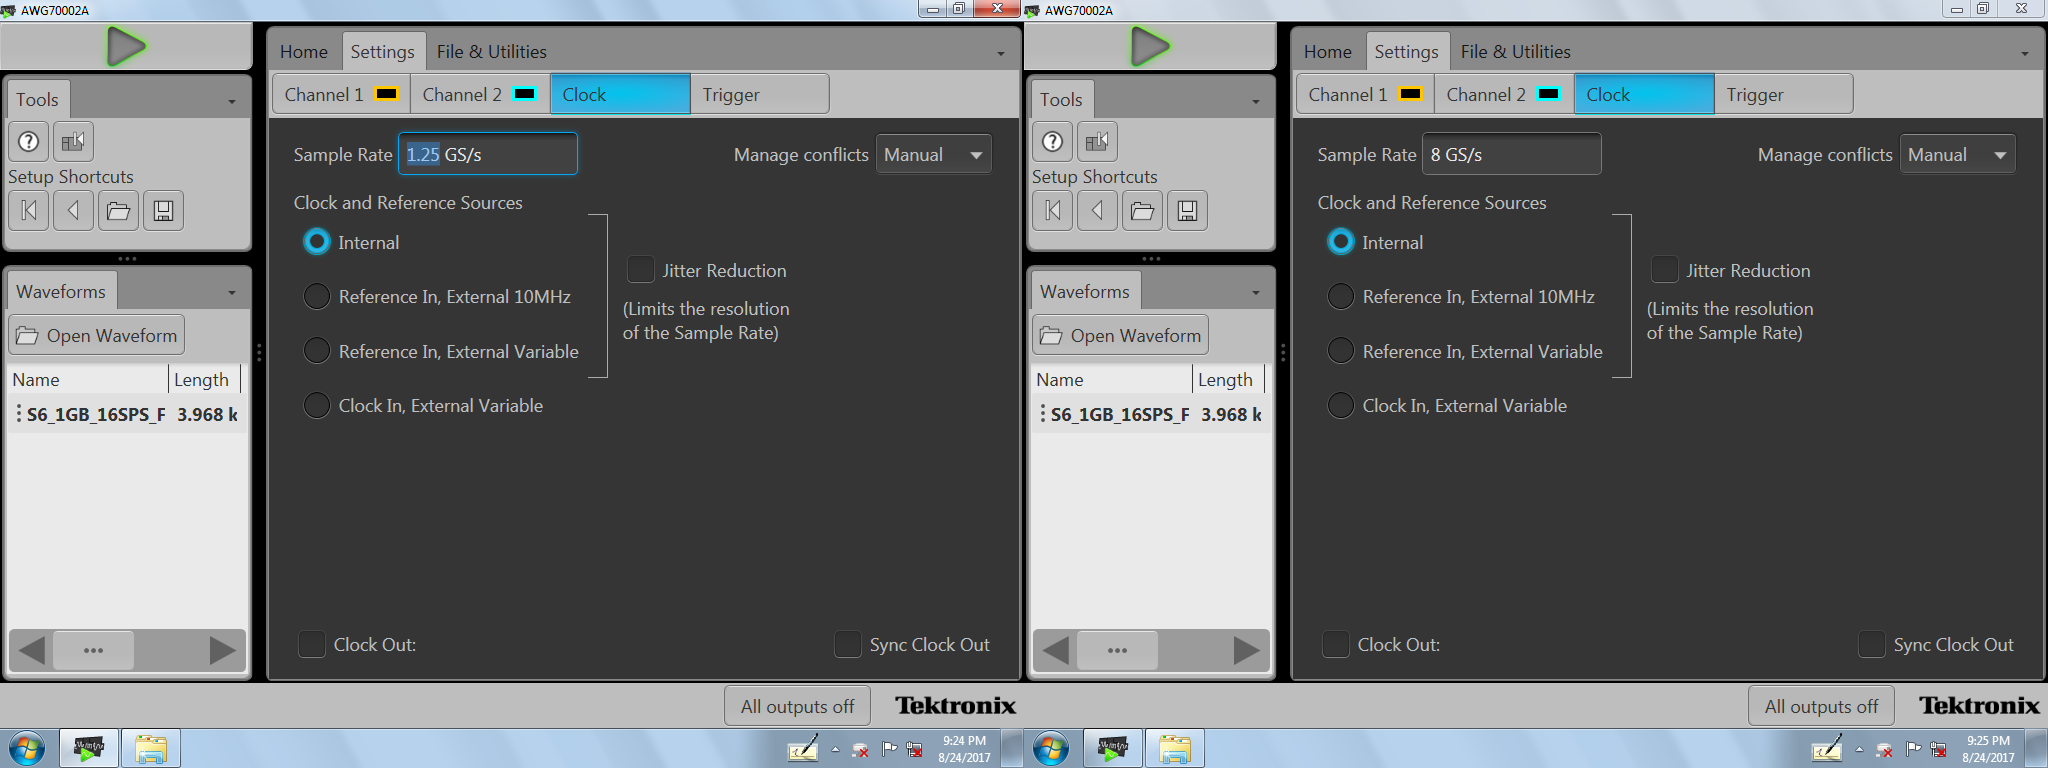
\includegraphics[width=\textwidth]{../mtools/sgnToWfm/figures/tutorial3}
	\label{TUT_ConfigSR}\caption{Configuring the right sampling rate}
\end{figure}
\bigskip

Compare the waveform in the AWG with the original signal, they should be identical (Figure 7.5).

\begin{figure}[h]
	\centering
	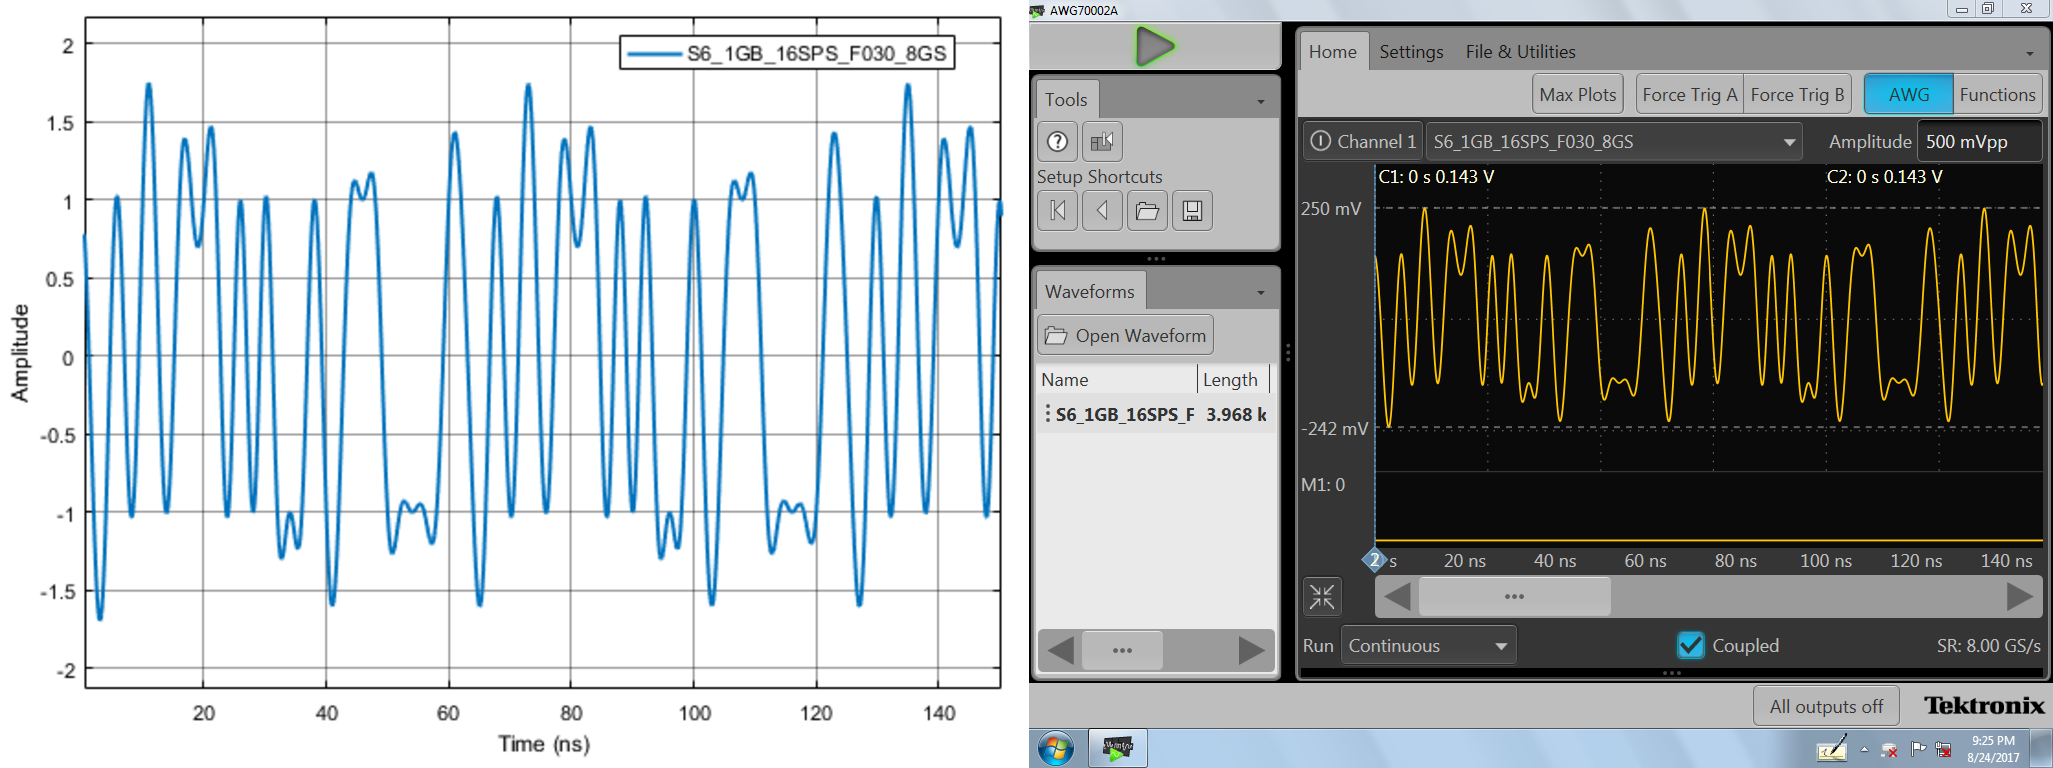
\includegraphics[width=\textwidth]{../mtools/sgnToWfm/figures/tutorial4}
	\label{TUT_CompGood}\caption{Comparison between the waveform in the AWG and the original signal after configuring the sampling rate}
\end{figure}
\bigskip

\noindent
\textbf{4. Generate the signal}: 
Output the wave by enabling the channel you want and clicking on the play button.


%\end{document} 